% Created by Jim Finnis
% Date Wed Feb 24 13:48:57 2021


\section{The data model}
The data model consists of two parts --- the data itself (largely
image cube data) and the graph. By far the most important kind of data
from the point of view of this document is the image data, which ties
into the user interface in complex ways. Other forms of data do exist,
but these are much simpler.

\subsection{ImageCube}
Most classes making up the image data 
model are described in the \texttt{pancamimage.py} file, including the main \texttt{ImageCube}
class. Some additional classes describing where images can come from are in \texttt{channelsource.py}.
The model is shown in outline in Fig.~\ref{image.png} although some links to channel sources
and mapping from nodes are omitted; these will be explained later.

\begin{figure}[ht]
\center
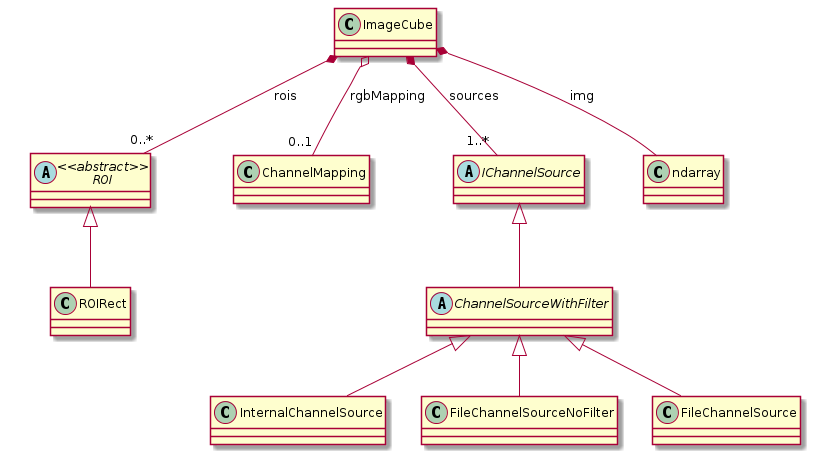
\includegraphics[width=5in]{image.png}
\caption{Outline UML class diagram of image model}
\label{image.png}
\end{figure}

The main class is \texttt{ImageCube}: this encapsulates a numpy array
\texttt{img}
which is the actual image data cube in the form
of a $w \times h \times depth$ array. The data type is 32-bit floating
point, and images are typically normalized to the range [0,1].

\subsection{IChannelSource and implementations}
Each \texttt{ImageCube} has a number of channels, and for each channel there must be a corresponding
entry in the \texttt{sources} list. This describes where that channel came from, so that (typically) filter
information can be preserved, where appropriate, through the graph. The sources for each channel are a set
of \texttt{IChannelSource} objects. For example, if an image was loaded through the RGB loader, it might
have three ``fake'' channel sources for red, green and blue. Thus the sources will be 
\begin{v}
[ {RED}, {GREEN}, {BLUE} ]
\end{v}
i.e.\ a list of three sets, each with a single source.
If the image is then converted to greyscale, this could
become
\begin{v}
[ {RED,GREEN,BLUE}, {RED,GREEN,BLUE}, {RED,GREEN,BLUE} ]
\end{v}
because each channel now contains information from the red, green and blue channels in the source file.
The \texttt{RED}, \texttt{GREEN} and \texttt{BLUE} values refer in this case to \texttt{FileChannelSourceNoFilter} objects
which contain ``fake'' filter information and a filename identifier.
Each \texttt{IChannelSource} contains methods for accessing:
\begin{itemize}
\item an \textbf{identifier string} for the source from which the channel was acquired (typically a filename or data ID);
\item a \textbf{filter} and methods for obtaining the filter name, filter position and an actual filter reference (for extra data such as centre wavelength) (note
that much of this information will be ``fake'' for images loaded from plain RGB files);
\item methods for getting string descriptors for this source.
\end{itemize}

Nodes generate and process this information in different ways. For example, a ``gradient'' node takes a single channel and converts it into an RGB image with
a colour gradient: here, the output image's sources are ``internal RGB'' sources with no identifier or sensible filter data because the output's colour
is entirely artificial. In contrast, a the ``curve'' for performing a sigmoid function on all channels of an image will give the output image the
same sources as the input image.

Sources are used to keep track of each channel as it moves through the graph so they can be processed and displayed appropriately:
Fig.~\ref{app.png} shows a typical node in the ``node controls and output'' section. This section, as it does in many nodes,
contains a ``canvas'' displaying an image. Above the canvas are three combo boxes which select the channels in the image cube to display on the canvas,
and these are typically labelled by a string generated from the source data for each channel (along with the index).

\subsection{RGB mappings}


\subsection{Regions of interest}
